\chapter{Evaluation}

In previous chapters, we've made fairly extensive reasoning behind each part of the algorithm. However, we have yet to see how the algorithm will perform as a whole. In this chapter, the algorithm is tested in various situations.

\section{Case Study}

First part of the evaluation consists of putting the algorithm up against handcrafted sets of obstacles. We can view how particular edge cases are handled, how natural the overall motion is, and if there are any situations it cannot reasonably deal with.

We can now demostrate initial results within a RoFI simulator. As a baseline, we consider a manipulator that consists of a chain of 4 modules, linked via the $-Z$ connectors. Since such a manipulator has 12 degrees of freedom, previous state of the art algorithms -- which mostly only scale up to 6 DoF -- would clearly not be useful.
The simulator does not consider the forces of gravity, or physical failure of the modules; these are aspects of further research. The reasoning behind using 4 modules as the baseline is that such a manipulator is flexible enough even though the joints are constrained, and with the state of the art hardware, it's feasible for the joint of a single module to lift the weight of around 3 connected modules, but not significantly more.

The measurements take place on consumer grade hardware, equipped with an Intel Core i7-8750H cpu.

To evaluate the quality of the algorithm, we want to explore how differently shaped environments affect the algorithm's runtime and ability to find successful paths.

As a sanity check, we can start with a simple case of a target near an obstacle, but reachable from the initial position. The environment is a wall made out of 12 small spheres. Figure~\ref{fig:sim3} shows the performed movement.

\begin{figure}
  \centering
  \begin{minipage}{\textwidth}
    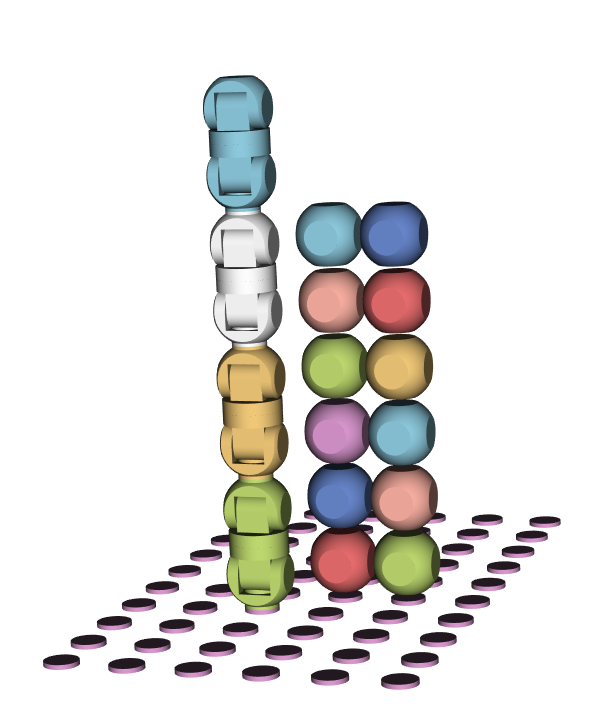
\includegraphics[width=0.24\textwidth]{sim3_0.png}
    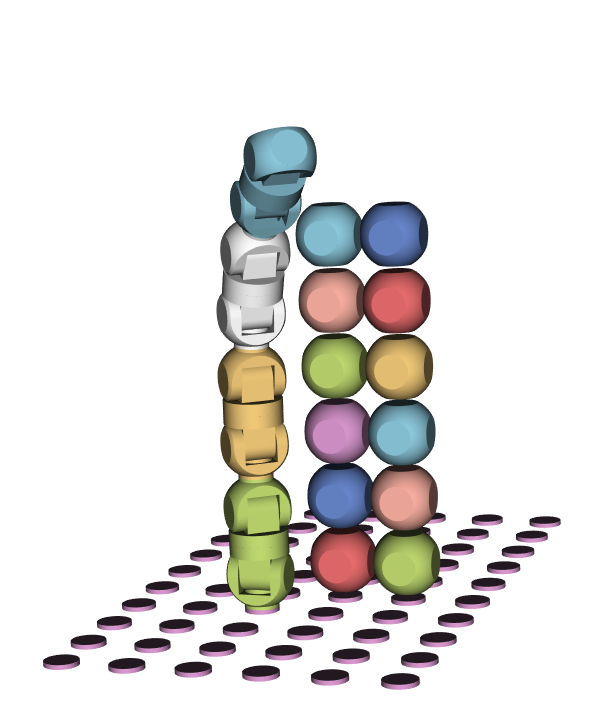
\includegraphics[width=0.24\textwidth]{sim3_1.png}
    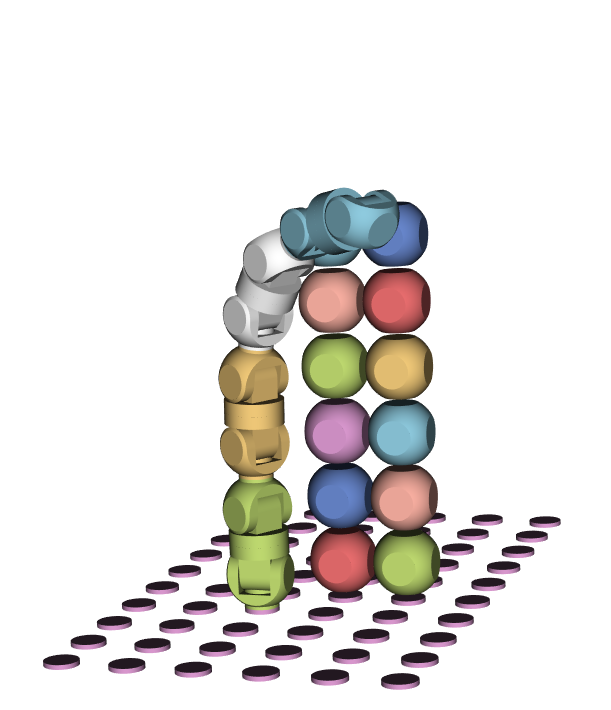
\includegraphics[width=0.24\textwidth]{sim3_2.png}
    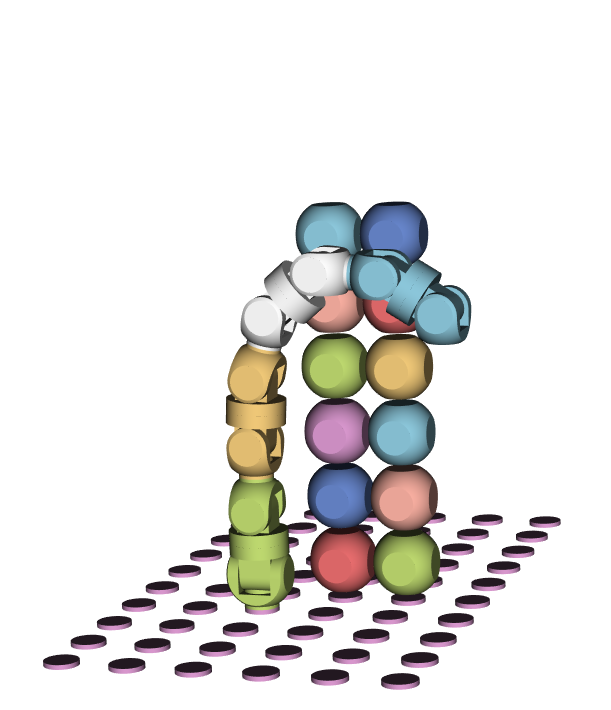
\includegraphics[width=0.24\textwidth]{sim3_3.png}
  \end{minipage}
  \caption{Test case 1: Target near obstacle}\label{fig:sim3}
\end{figure}

A notable feature observable in this case is that even though there is a fairly high number of obstacles, they don't affect the final result in a negative way unless they are in the way. The final position looks very natural, and the performed movement is as smooth as it gets: a direct interpolation between the initial and target position. Since the target is visible from the initial position, the algorithm directly finds the path from it to the target. The whole computation runs for around $0.07$ seconds.

A more interesting case is observable when we start off in a position close to the wall and try to reach a target behind the wall. In this case, the algorithm needs to first move back to avoid the wall, and then go to the target. The direct path can no longer be taken due to the obstacles, and going around the wall is infeasible due to the limited length of the manipulator. The resulting motion can be seen in Figure~\ref{fig:sim4}.

\begin{figure}[h]
  \centering
  \begin{minipage}{\textwidth}
    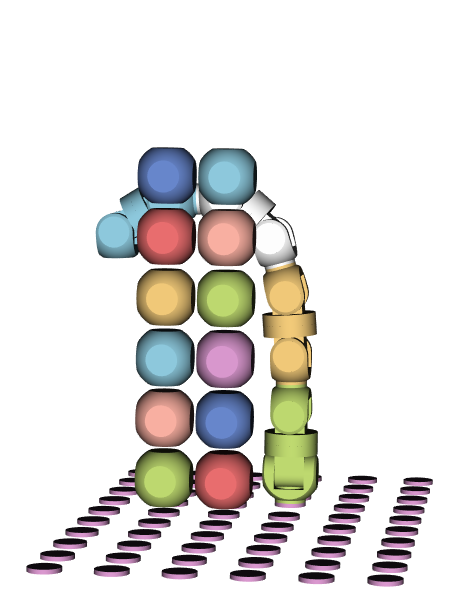
\includegraphics[width=0.24\textwidth]{sim4_0.png}
    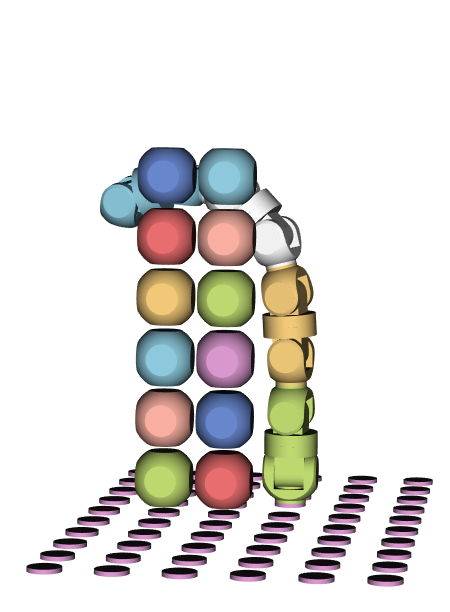
\includegraphics[width=0.24\textwidth]{sim4_1.png}
    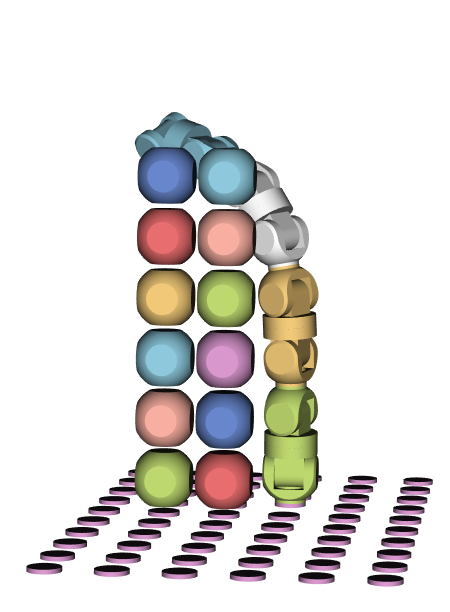
\includegraphics[width=0.24\textwidth]{sim4_2.png}
    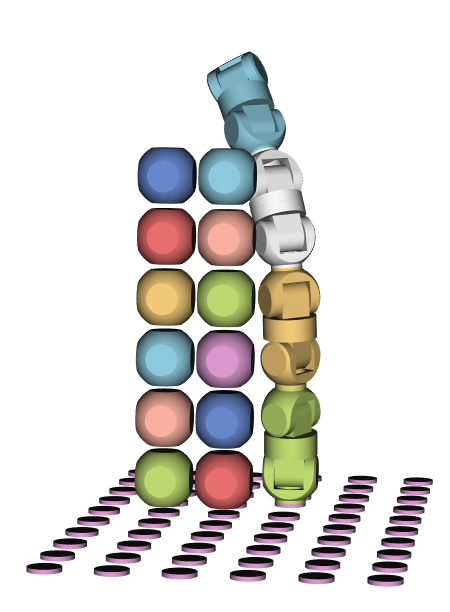
\includegraphics[width=0.24\textwidth]{sim4_3.png}

    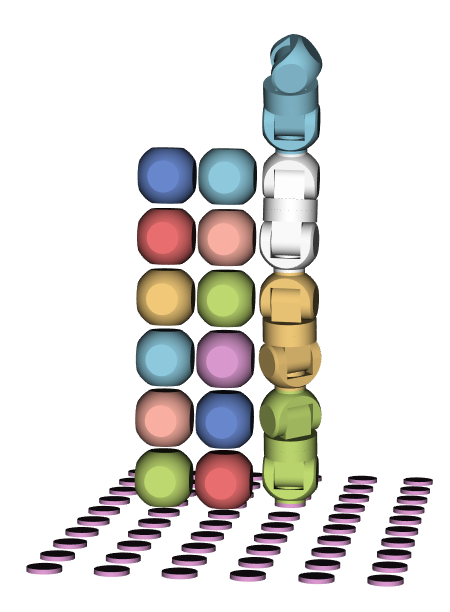
\includegraphics[width=0.24\textwidth]{sim4_4.png}
    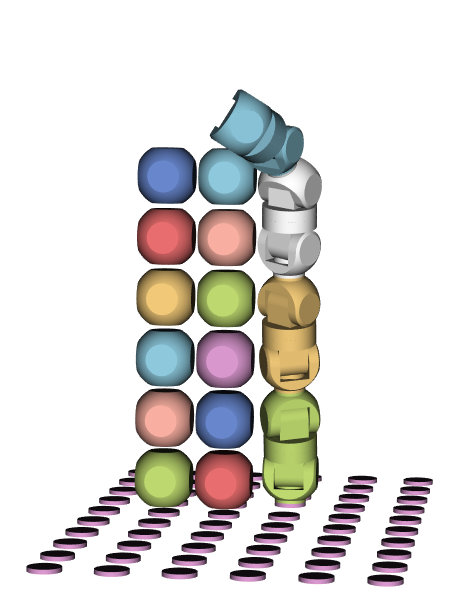
\includegraphics[width=0.24\textwidth]{sim4_5.png}
    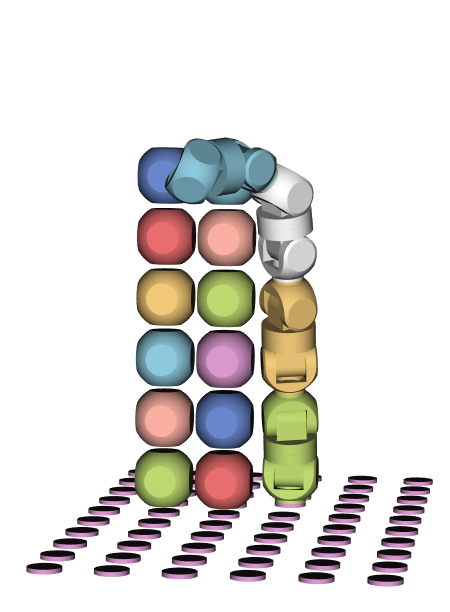
\includegraphics[width=0.24\textwidth]{sim4_6.png}
    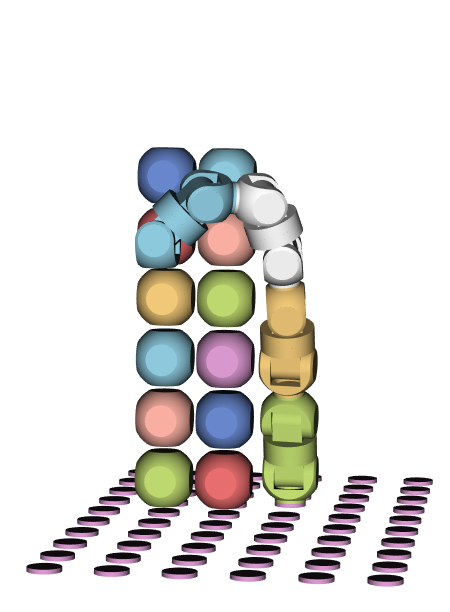
\includegraphics[width=0.24\textwidth]{sim4_7.png}
  \end{minipage}
  \caption{Test case 2: Target behind obstacle}\label{fig:sim4}
\end{figure}

Unlike the first test case, the algorithm doesn't immediately find the right path. Since the paths that lead behind the wall are physically closer, they are evaluated as shorter at first, but trying to folow them fails due to the limited length of the manipulator. On the 5\th{} path, a correct solution that goes around the wall is found. Since we needed to explore multiple paths, each of which is associated with a lot of computation, the solution was found in $0.5$ seconds.

The next test case consists of trying to fit the manipulator in a small hole between obstacles and reach a target behind it. The problem has proven to be the most challenging one yet. Any path to the target has to go through the hole, but the direction where we come from plays a part as well: in order to fit the joints through the hole, the manipulator needs to move in a very specific direction. Eventually, it does find a solution, see Figure~\ref{fig:sim5}. However, if even one path that containing the point between the obstacles fails, the cost on it is raised and the impossible paths around the obstacle are tried instead. There are, of course, ways to address this issue, but since we want to keep the algorithm as general as possible, they were not implemented.

\begin{figure}[h]
  \centering
  \begin{minipage}{\textwidth}
    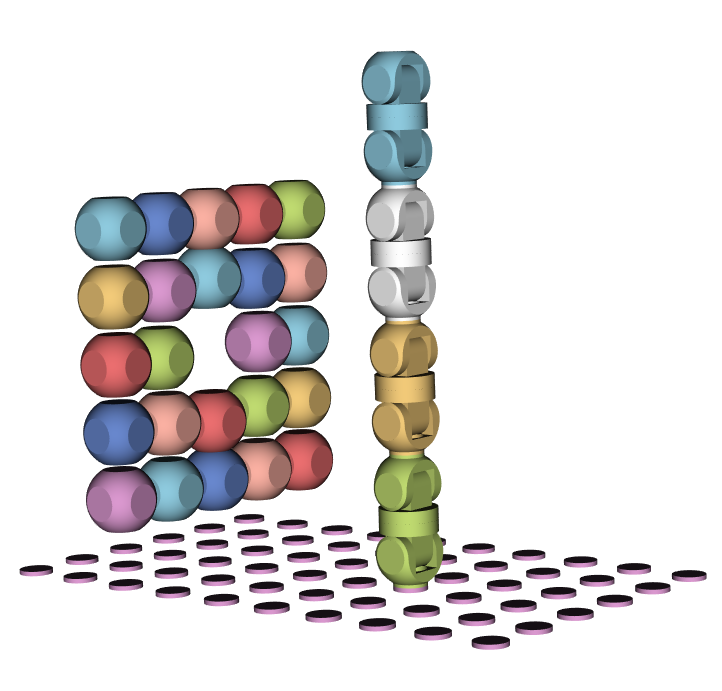
\includegraphics[width=0.24\textwidth]{sim5_0.png}
    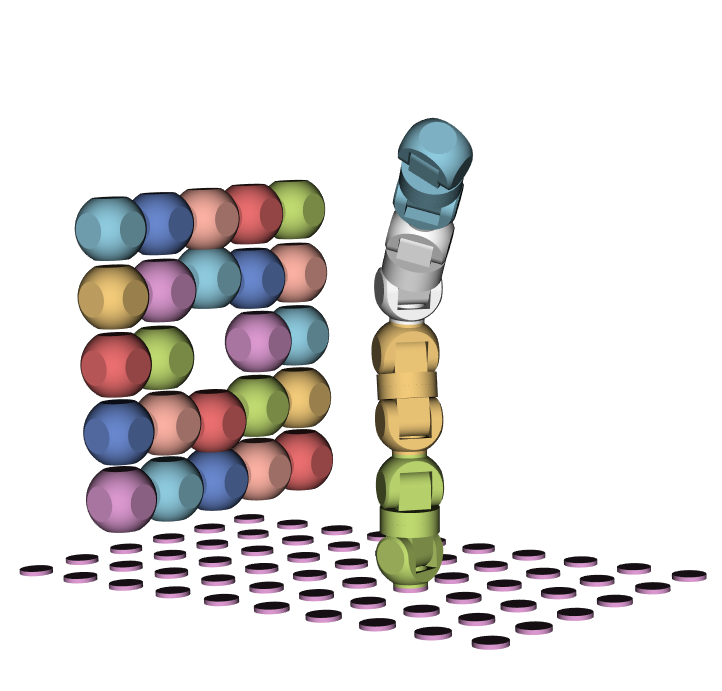
\includegraphics[width=0.24\textwidth]{sim5_1.png}
    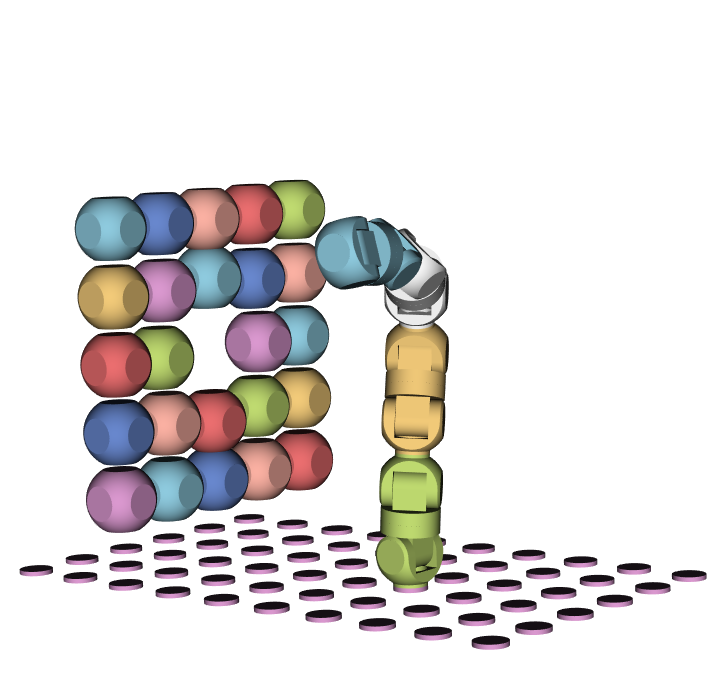
\includegraphics[width=0.24\textwidth]{sim5_2.png}
    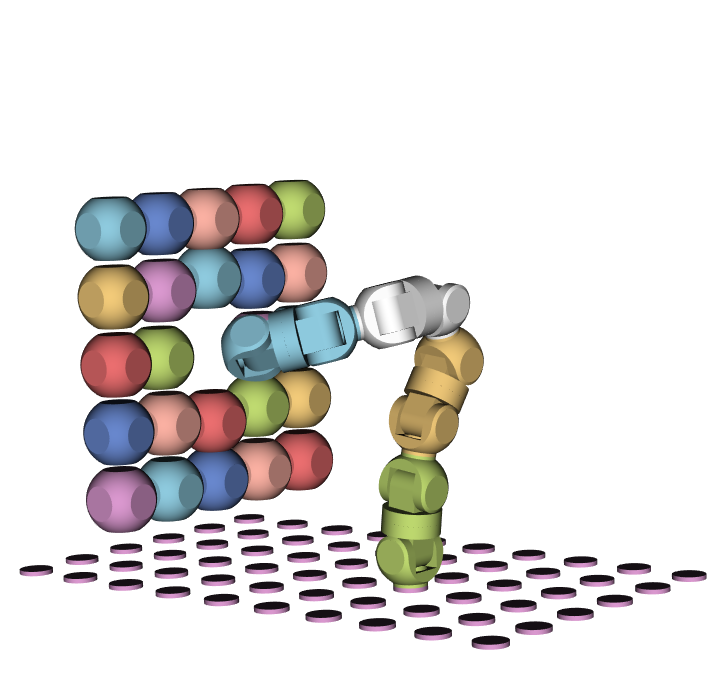
\includegraphics[width=0.24\textwidth]{sim5_3.png}

    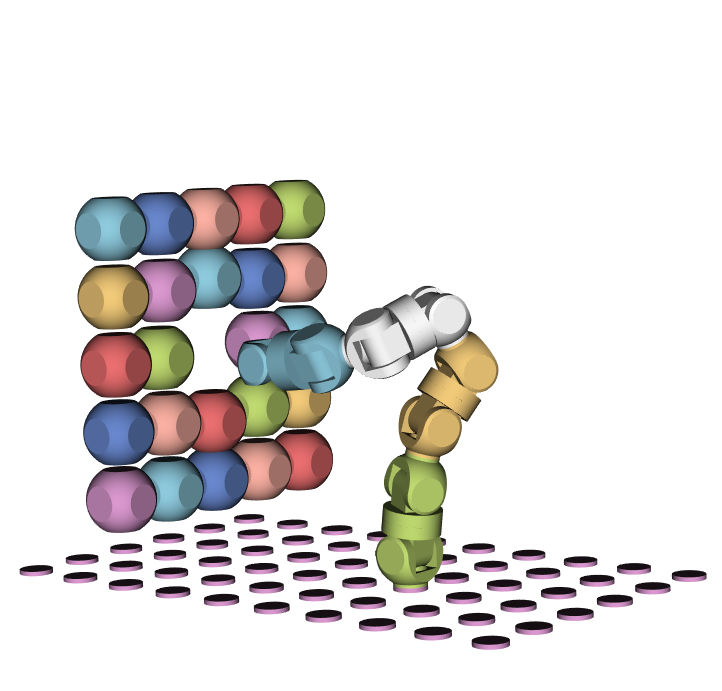
\includegraphics[width=0.24\textwidth]{sim5_4.png}
    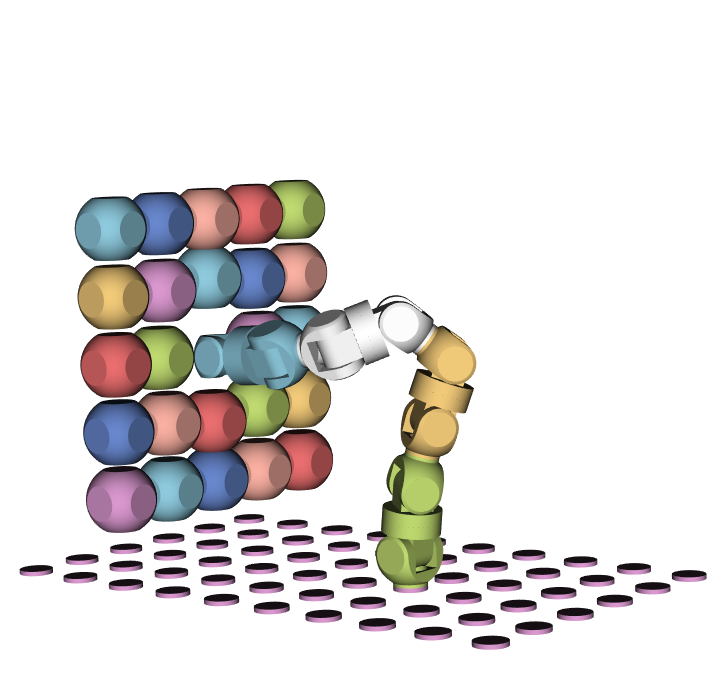
\includegraphics[width=0.24\textwidth]{sim5_5.png}
    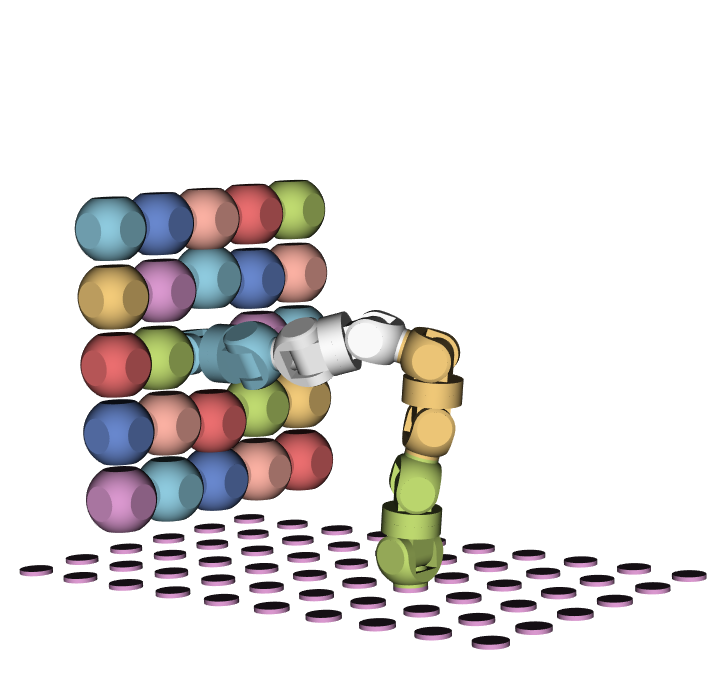
\includegraphics[width=0.24\textwidth]{sim5_6.png}
    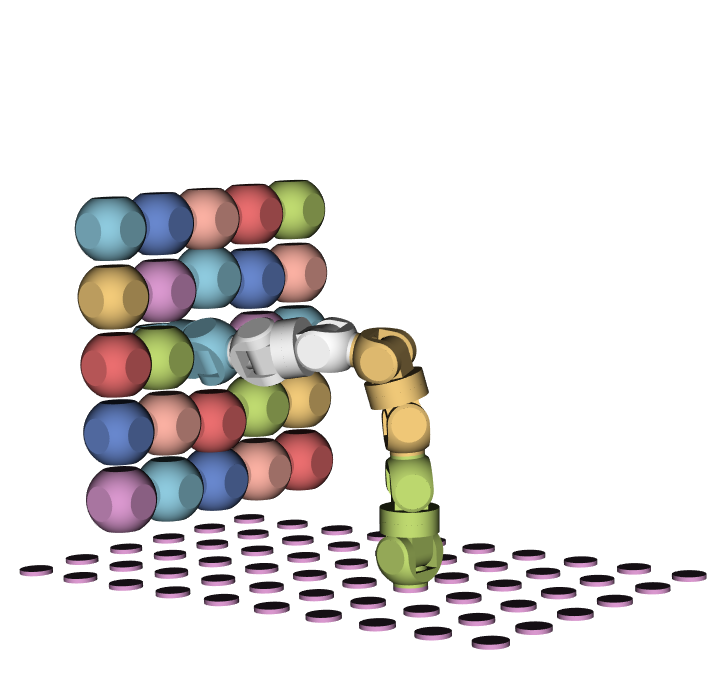
\includegraphics[width=0.24\textwidth]{sim5_7.png}
  \end{minipage}
  \caption{Test case 3: Hole between obstacles}\label{fig:sim5}
\end{figure}

Depending on how far beyond the hole the target is, the number of explored paths is anywhere from $10$ to $37$. Depending on the number of paths, the computation times range between $1$ and $6$ seconds.

\section{Performance}

This section is about benchmarking the algorithm.
